\documentclass[12pt]{article}
\usepackage[utf8]{inputenc}
\usepackage[margin=1in]{geometry}
\usepackage[spanish]{babel}\decimalpoint
\usepackage{setspace}\onehalfspacing
\usepackage{parskip} % Espacio entre parrafos.
\usepackage{graphicx} % Para usar comando \includegraphics[]{}
\usepackage{amssymb} % Para usar el simbolo del conj. de los Reales.
\usepackage{amsmath} % Para usar columnas vectoriales.
\usepackage{multirow} % Para unir multiples filas en una tabla.
\usepackage{hyperref} % Siempre debe ser el ultimo paquete.


\setcounter{tocdepth}{2} % Que no incluya subsubsections en la tabla de contenidos (toc).

%================================

\title{Clase 3. Matrices y la Matriz Inversa.}
\author{MIT 18.02: Multivariable Calculus.}
\date{}


\begin{document}

\maketitle

\begin{abstract}
\noindent Iniciamos esta clase viendo un último ejemplo donde ocupamos tanto los determinantes como el producto cruz y, en el resto de ella, nos centraremos en estudiar de forma introductoria a las matrices y, en particular, a la matriz inversa.
\end{abstract}


\section{Matrices.}

Sea el punto $P = (x_{1}, \ x_{2}, \ x_{3})$, el cual se encuentra en el siguiente espacio de coordenadas.

\begin{figure}[hbt!]
\centering
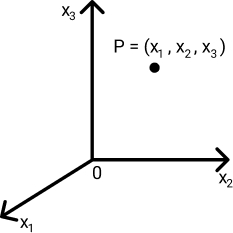
\includegraphics[scale=0.6]{img/matrices-1.jpg}
\end{figure}

Suponga que, por necesidad, cambiamos las coordenadas del espacio y el punto $P$ queda ubicado en $(u_{1}, \ u_{2}, \ u_{3})$.

\newpage

\begin{figure}[hbt!]
\centering
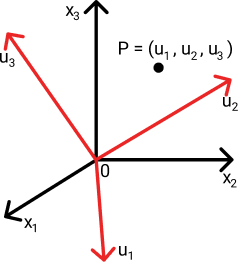
\includegraphics[scale=0.6]{img/matrices-2.jpg}
\end{figure}

Las coordenadas $u_{1}$, $u_{2}$ y $u_{3}$ podemos expresarlas en función de $x_{1}$, $x_{2}$ y $x_{3}$ como el de a continuación:
\[
\left\{
\begin{aligned}
2x_{1} + 3x_{2} + 3x_{3} &= u_{1} \\
2x_{1} + 4x_{2} + 5x_{3} &= u_{2} \\
x_{1} + x_{2} + 2x_{3} &= u_{3}
\end{aligned}
\right.
\]
El sistema de ecuaciones de arriba podemos escribirlo como el siguiente \textbf{producto matricial}:
\[
  \mathbf{A}\mathbf{x} = \mathbf{u}
\]
donde:
\begin{align*}
\mathbf{A} &=
\begin{bmatrix}
2 & 3 & 3 \\
2 & 4 & 5 \\
1 & 1 & 2
\end{bmatrix} &
\mathbf{x} &=
\begin{bmatrix}
x_{1} \\ x_{2} \\ x_{3}
\end{bmatrix} &
\mathbf{u} &=
\begin{bmatrix}
u_{1} \\ u_{2} \\ u_{3}
\end{bmatrix} &
\end{align*}
La matriz $\mathbf{A}$ se conoce como \textbf{matriz de coeficientes}, ya que contiene las constantes o coeficientes del sistema de ecuaciones, mientras que los vectores $\mathbf{x}$ y $\mathbf{u}$ reciben el nombre de \textbf{vectores columna}.

En general y como acabamos de ver, una \textbf{matriz} es simplemente un arreglo rectangular de números, símbolos o expresiones ordenados en filas y columnas.

Cuando trabajamos con matrices, es habitual señalar su dimensión en la forma $n \times m$, donde $n$ indica la cantidad de filas y $m$ la de columnas. Para el caso de $\mathbf{A}$, podemos ver que es de $3 \times 3$ dimensiones y, al ser $n = m$, recibe el nombre de \textbf{Matriz Cuadrada}. Si $n \neq m$, entonces se la categoriza como \textbf{Matriz Rectangular}.

Las \textbf{filas} y \textbf{columnas} de una matriz también se suelen interpretar como vectores. Los primeros reciben el nombre de \textbf{vectores fila} y son de $1 \times m$ dimensiones, mientras que los segundos se conocen como \textbf{vectores columna} y son de $n \times 1$ dimensiones. Como vimos, los vectores $\mathbf{x}$ y $\mathbf{u}$ corresponde a estos últimos, ya que son de $3 \times 1$.

Al trabajar de forma algebraica con una matriz $\mathbf{B}$ cualquiera, sus entradas se denotan en la forma $b_{i, j}$, donde $i$ es el número de fila en el que se encuentra $b$ y $j$ el número de columna. El conteo se hace de arriba hacia abajo para $i$ y de izquierda a derecha para $j$. Por ejemplo, la entrada $a_{2, 3} = 5$ en $\mathbf{A}$ porque dicho valor está en su segunda fila y tercera columna.

Un conjunto de \textbf{matrices} son \textbf{iguales} si sus \textbf{dimensiones y entradas} también lo son.

\subsection{Operaciones aritméticas con y entre matrices.}

\subsubsection{Adición y sustracción entre matrices.}

Es posible \textbf{sumar y restar matrices} solo si son de \textbf{dimensiones iguales}. Cuando se cumple dicho requisito, aplicamos dichas operaciones entre las entradas de ellas y resulta en una nueva matriz.

Formalmente, sean dos matrices $\mathbf{V} = [v_{i, j}]$ y $\mathbf{W} = [w_{i, j}]$ de iguales dimensiones. Entonces:
\[
  \mathbf{V} \pm \mathbf{W} = [v_{i, j} \pm w_{i, j}]
\]
Por ejemplo:
\[
\begin{bmatrix}
1 & 4 \\
3 & 5
\end{bmatrix} +
\begin{bmatrix}
2 & 1 \\
9 & 6
\end{bmatrix} =
\begin{bmatrix}
1 + 2 & 4 + 1 \\
3 + 9 & 5 + 6
\end{bmatrix} =
\begin{bmatrix}
3 & 5 \\
12 & 11
\end{bmatrix}
\]

\subsubsection{Multiplicación escalar de una matriz.}

Al igual que al trabajar con vectores, la \textbf{multiplicación entre un escalar a una matriz} corresponde al producto entre dicho número y cada entrada de esta última.
\[
  c \cdot \mathbf{W} = [c \cdot w_{i, j}] \qquad (c = \text{constante})
\]

\subsubsection{Producto matricial.}

El \textbf{producto matricial} o producto entre matrices es más restrictivo. Se puede realizar siempre que \textbf{la cantidad de columnas de la matriz de la izquierda sea igual a la cantidad de filas de la ubicada a la derecha}, puesto que es equivalente al \textbf{producto punto} entre los vectores fila de la primera y los vectores columna de la segunda.

Por ejemplo, sean dos matrices:
\[
\mathbf{W} =
\begin{bmatrix}
w_{1, 1} & w_{1, 2} \\
w_{2, 1} & w_{2, 2}
\end{bmatrix}
\qquad
\mathbf{V} =
\begin{bmatrix}
v_{1, 1} & v_{1, 2} \\
v_{2, 1} & v_{2, 2}
\end{bmatrix}
\]
entonces:
\[
\mathbf{W} \cdot \mathbf{V} =
\begin{bmatrix}
(w_{1, 1} \cdot v_{1, 1}) + (w_{1, 2} \cdot v_{2, 1}) & (w_{1, 1} \cdot v_{1, 2}) + (w_{1, 2} \cdot v_{2, 2}) \\
(w_{2, 1} \cdot v_{1, 1}) + (w_{2, 2} \cdot v_{2, 1}) & (w_{2, 1} \cdot v_{1, 2}) + (w_{2, 2} \cdot v_{2, 2})
\end{bmatrix}
\]
En general, se cumple que si $\mathbf{W}$ es de $k \times m$ y $\mathbf{V}$ es de $m \times p$, entonces $\mathbf{W} \cdot \mathbf{V}$ será una matriz de $k \times p$ dimensiones.

Por otra parte, el producto matricial representa la \textbf{transformación lineal} de la matriz ubicada en la derecha a partir de la que está en la izquierda. Por ejemplo, en $\mathbf{V}\mathbf{W}$ se refiere a que pasamos a $\mathbf{W} \to \mathbf{V}\mathbf{W}$ por medio de $\mathbf{V}$.

Otro ejemplo de una transformación lineal, es el producto matricial que vimos al inicio de esta sección:
\[
  \mathbf{A} \cdot \mathbf{x} = \mathbf{u}
\]
Como vemos, podemos interpretar la operación de arriba como haber transformado a $\mathbf{x} \to \mathbf{u}$ a partir de la matriz $\mathbf{A}$. Además, la ecuación se cumple porque $\mathbf{A}$ es de $3 \times 3$ y $\mathbf{x}$ es de $3 \times 1$, lo que implica que $\mathbf{u}$ debe ser de $3 \times 1$, lo cual vimos que es verdadero.

Ahora, suponga que es posible calcular el producto entre las matrices $\mathbf{V}$, $\mathbf{W}$ y $\mathbf{Z}$. De ellas es posible obtener las siguientes \textbf{propiedades} de esta operación:
\begin{align*}
&\text{Asociativa} \rightarrow \mathbf{V}(\mathbf{W}\mathbf{Z}) = (\mathbf{V}\mathbf{W}) \mathbf{Z} \\
&\text{Distributiva (1)} \rightarrow \mathbf{V} (\mathbf{W} + \mathbf{Z}) = \mathbf{V}\mathbf{W} + \mathbf{V}\mathbf{Z} \\
&\text{Distributiva (2)} \rightarrow (\mathbf{W} + \mathbf{Z}) \mathbf{V} = \mathbf{W}\mathbf{V} + \mathbf{Z}\mathbf{V}
\end{align*}
Separamos la propiedad distributiva en dos partes, porque el \textbf{orden de los factores importa} en la multiplicación entre matrices. Esto se debe, principalmente, a la condición de las dimensiones de una y otra. Es por ello que \textbf{no necesariamente existe la propiedad conmutativa} en esta operación. Es decir:
\[
  \mathbf{V}\mathbf{W} \neq \mathbf{W}\mathbf{V}
\]
La propiedad conmutativa se da solo en un caso, el cual revisaremos más adelante.


\subsection{Matriz Identidad.}

Es posible encontrar distintos tipos de matrices y una de ellas es la \textbf{Matriz Identidad} $\mathbf{I}$, la cual se caracteriza por ser \textbf{cuadrada} y porque su diagonal principal\footnote{Es decir, las entradas que van en diagonal desde la esquina superior izquierda hasta la esquina inferior derecha.} consiste solo de unos y el resto son ceros. Por ejemplo, a continuación tenemos una de $3 \times 3$.
\[
\mathbf{I} =
\begin{bmatrix}
1 & 0 & 0 \\
0 & 1 & 0 \\
0 & 0 & 1
\end{bmatrix}
\]
La matriz identidad suele ser muy buscada al trabajar con matrices, porque corresponde a un \textbf{neutro multiplicativo}. Es decir, sean dos matrices $\mathbf{V}$ de $k \times n$ y $\mathbf{I}$ de $n \times n$, entonces:
\[
  \mathbf{V} \cdot \mathbf{I} = \mathbf{V}
\]
Un ejemplo donde podemos encontrarnos una matriz identidad, es en la siguiente matriz de rotación $\mathbf{R}$.
\[
\mathbf{R} =
\begin{bmatrix}
0 & -1 \\
1 & 0
\end{bmatrix}
\]
La matriz $\mathbf{R}$ permite hacer rotar objetos (sean matrices o vectores) de dos filas en $90^{\circ}$ en dirección contra las manillas del reloj. Por ejemplo:
\[
\begin{bmatrix}
0 & -1 \\
1 & 0
\end{bmatrix}
\cdot
\begin{bmatrix} x \\ y \end{bmatrix} =
\begin{bmatrix} -y \\ x \end{bmatrix}
\]
Lo interesante es que si multiplicamos a $\mathbf{R}$ por sí misma, obtenemos a $-\mathbf{I}$,
\[
\mathbf{R} \cdot \mathbf{R} =
\begin{bmatrix}
0 & -1 \\
1 & 0
\end{bmatrix} \cdot
\begin{bmatrix}
0 & -1 \\
1 & 0
\end{bmatrix} =
\begin{bmatrix}
-1 & 0 \\
0 & -1
\end{bmatrix} =
- \mathbf{I}
\]
donde $-\mathbf{I}$ corresponde a una matriz de rotación que hace girar a objetos con respecto a su eje en $180^{\circ}$ en dirección contra las manillas del reloj.


\subsection{Matriz Inversa.}

Hemos señalado que la ecuación $\mathbf{A}\mathbf{x} = \mathbf{u}$ representa la transformación lineal de $\mathbf{x}$ a $\mathbf{u}$ a partir de $\mathbf{A}$. En ciertas ocasiones es posible hacer el trabajo inverso, pasando a $\mathbf{u} \to \mathbf{x}$ por medio de una matriz denotada como $\mathbf{A}^{-1}$ y que recibe el nombre de \textbf{Matriz Inversa} de $\mathbf{A}$.

Las matrices inversas solo existen en \textbf{matrices cuadradas}. Es decir, $\mathbf{A}$ debe ser de $n \times n$ para que exista $\mathbf{A}^{-1}$.

Ahora bien, si $\mathbf{A}$ es de $n \times n$, la \textbf{principal condición} para que exista $\mathbf{A}^{-1}$ es que:
\[
  \mathbf{A}^{-1}\mathbf{A} = \mathbf{A}\mathbf{A}^{-1} = \mathbf{I}
\]
Lo que nos muestra la igualdad de arriba es que, cuando existe $\mathbf{A}^{-1}$, podemos revertir o anular la transformación realizada por medio de $\mathbf{A}$ al ser multiplicada por su inversa, ya que termina siendo igual a $\mathbf{I}$ y lo mismo ocurre en sentido contrario, revirtiendo la transformación realizada por $\mathbf{A}^{-1}$ al ser multiplicada por $\mathbf{A}$.

La matriz inversa es muy buscada, porque nos permite \textbf{encontrar las soluciones de un sistema de ecuaciones lineales}. En particular, si multiplicamos al sistema $\mathbf{A}\mathbf{x} = \mathbf{u}$ por $\mathbf{A}^{-1}$, entonces:
\begin{align*}
\mathbf{A}^{-1}(\mathbf{A}\mathbf{x}) &= \mathbf{A}^{-1}\mathbf{u} \\
(\mathbf{A}^{-1}\mathbf{A})\mathbf{x} &= \mathbf{A}^{-1}\mathbf{u} \\
\mathbf{I}\mathbf{x} &= \mathbf{A}^{-1}\mathbf{u} \\
\mathbf{x} &= \mathbf{A}^{-1}\mathbf{u}
\end{align*}
Por lo tanto, si existe $\mathbf{A}^{-1}$ y conocemos los valores de $\mathbf{u}$, podemos encontrar las soluciones contenidas en $\mathbf{x}$ transformando (o revirtiendo) de $\mathbf{u} \to \mathbf{x}$ a partir de $\mathbf{A}^{-1}$.

\subsubsection{Calculando una Matriz Inversa para matrices pequeñas.}

Existen distintas formas para encontrar la inversa de una matriz cuadrada (cuando existe). Acá veremos una que es eficiente cuando es de menor tamaño\footnote{Para aquellas de mayor tamaño, es más eficiente obtenerlas por medio del Método (o algoritmo) de Eliminación de Gauss, que estudiamos con mayor detalle en Álgebra Lineal.}.

Como recordaremos, las columnas de una matriz podemos interpretarlas como vectores fila. Es decir, podemos conformar una matriz a partir de ellos. Por lo tanto, también podemos calcular el determinante de igual manera a como lo estudiamos en la clase anterior.

\newpage

En general, en \textbf{toda matriz cuadrada} es posible calcular su determinante. Para el caso de las de $2 \times 2$, lo calculamos como:
\[
\det(\mathbf{A}) =
\begin{vmatrix}
a_{1,1} & a_{1,2} \\
a_{2,1} & a_{2,2}
\end{vmatrix} =
a_{1,1}a_{2,2} - a_{1,2}a_{2,1};
\qquad
\text{donde }
\mathbf{A} =
\begin{bmatrix}
a_{1,1} & a_{1,2} \\
a_{2,1} & a_{2,2}
\end{bmatrix}
\]
Para una matriz de $n \times n$, con $n > 2$, obtenemos su determinante a partir de un proceso conocido como \textbf{expansión} por una columna o fila de ella. Consiste en la suma de las productos entre cada entrada de la fila o columna que decidimos expandir y un valor conocido como \textbf{Cofactor}, que se denota como $C_{i, j}$.

Por ejemplo, a continuación tenemos el determinante de una $\mathbf{A}$ de $3 \times 3$ expandida por su segunda columna.
\[
\det(\mathbf{A}) =
\begin{vmatrix}
a_{1,1} & a_{1,2} & a_{1,3} \\
a_{2,1} & a_{2,2} & a_{2,3} \\
a_{3,1} & a_{3,2} & a_{3,3}
\end{vmatrix} =
a_{1,2} \cdot C_{1,2} + a_{2,2} \cdot C_{2,2} + a_{3,2} \cdot C_{3,2}
\]
donde:
\[
\mathbf{A} =
\begin{bmatrix}
a_{1,1} & a_{1,2} & a_{1,3} \\
a_{2,1} & a_{2,2} & a_{2,3} \\
a_{3,1} & a_{3,2} & a_{3,3}
\end{bmatrix}
\]
Cuando expandimos por la segunda columna, para cada entrada de ella es posible formar determinantes de $2 \times 2$, los cuales se conocen como \textbf{Menores} (\textit{Minors}, en inglés) y que se denota como $M_{i, j}$. Por ejemplo, al expandir a $\mathbf{A}$ por su segunda columna, el menor $M_{3, 2}$ corresponde a:
\[
M_{3, 2} =
\begin{vmatrix}
a_{1,1} & a_{1,3} \\
a_{2,1} & a_{2,3}
\end{vmatrix}
\]
puesto está conformado por las entradas de $\mathbf{A}$ que no están en negrita, que son las que sobran de la expansión.
\[
\mathbf{A} =
\begin{bmatrix}
a_{1,1} & \mathbf{a_{1,2}} & a_{1,3} \\
a_{2,1} & \mathbf{a_{2,2}} & a_{2,3} \\
\mathbf{a_{3,1}} & \mathbf{a_{3,2}} & \mathbf{a_{3,3}}
\end{bmatrix}
\]
En ese sentido, el \textbf{cofactor} $C_{i,j}$ es el producto entre $(-1)^{i + j}$ y el valor de su menor $M_{i, j}$ correspondiente.
\[
  C_{i, j} = (-1)^{i + j} \cdot M_{i, j}
\]
Por lo tanto, podemos reescribir la fórmula del determinante de $\mathbf{A}$ expandido por su segunda fila como:
\[
\det(\mathbf{A}) =
\begin{vmatrix}
a_{1,1} & a_{1,2} & a_{1,3} \\
a_{2,1} & a_{2,2} & a_{2,3} \\
a_{3,1} & a_{3,2} & a_{3,3}
\end{vmatrix} =
a_{1,2} \cdot (-1)^{1 + 2}M_{1 + 2} + a_{2,2} \cdot (-1)^{2 + 2}M_{2 + 2} + a_{3,2} \cdot (-1)^{3 + 2}M_{3 + 2}
\]
Con los cofactores $C_{i, j}$ es posible conformar una matriz conocida como \textbf{Matriz de Cofactores} denotada como $\mathbf{C}$.

Ahora que sabemos calcular el determinante de una matriz de $n \times n$ y que conocemos a la matriz de cofactores $\mathbf{C}$, podemos ver cómo se calcula la inversa de una matriz.

Si $\mathbf{A}$ es una matriz cuadrada e invertible, su inversa $\mathbf{A}^{-1}$ podemos conocerla como el producto entre el recíproco de su determinante y la \textbf{Matriz Adjunta} de $\mathbf{A}$, que se denota como Adj($\mathbf{A}$).
\[
  \mathbf{A}^{-1} = \frac{1}{\det(\mathbf{A})} \cdot \text{Adj}(\mathbf{A})
\]
La \textbf{Transposición} es la operación de pasar las filas a columnas o viceversa de una matriz o vector y se suele denotar como $\mathbf{A}^{T}$ o $\mathbf{A'}$. A continuación tenemos dos ejemplos que la ilustran.
\begin{align*}
\mathbf{A} &=
\begin{bmatrix}
4 & 1 & 3 \\
5 & 7 & 2
\end{bmatrix}
\Rightarrow
\mathbf{A}^{T} =
\begin{bmatrix}
4 & 5 \\
1 & 7 \\
3 & 2
\end{bmatrix} &
\mathbf{b} &=
\begin{bmatrix}
2 & 5 & 1
\end{bmatrix}
\Rightarrow
\mathbf{b}^{T} =
\begin{bmatrix}
2 \\ 5 \\ 1
\end{bmatrix}
\end{align*}
Hemos señalado la transposición porque la \textbf{Matriz Adjunta} de $\mathbf{A}$, Adj$(\mathbf{A})$, corresponde a \textbf{matriz de cofactores transpuesta} denotada como $\mathbf{C}^{T}$. Por lo tanto, la fórmula de la matriz inversa de $\mathbf{A}^{-1}$ podemos reescribirla como:
\[
  \mathbf{A}^{-1} = \frac{1}{\det(\mathbf{A})} \cdot \mathbf{C}^{T}
\]
Esta fórmula implica, además, que si el $\det(\mathbf{A}) = 0$, entonces $\mathbf{A}^{-1}$ \textbf{NO existe}.

\end{document}
